%Base Content generated with the help of AI.

\documentclass{beamer}
\usepackage{listings}
\usepackage{graphicx}
\usepackage{svg}
\usepackage{textcomp}
% Presentation theme
\usetheme{default}
\usecolortheme{seagull}
% Listings settings for code display
\lstset{
    basicstyle=\ttfamily,
    columns=fullflexible,
    frame=single,
    breaklines=true
}
% Title slide
\title{\LaTeX\ and why you should, too!}
\author{Prof. Jeff Tithof \inst{1} \and Dean Maxam \inst{1} \and Yusra Farhat Ullah \inst{1}}
\institute{\inst{1} Department of Mechanical Engineering, University of Minnesota - Twin Cities}
\date{\today}


\begin{document}

\begin{frame}
    \titlepage
\end{frame}

\begin{frame}{What is \LaTeX{}}
\begin{itemize}
    \item Typesetting software for document preparation (particularly academic)
    \item Developed by Leslie Lamport in 1984, based on TeX typesetting language by Donald Knuth
    \item Free and openly licensed, cross-platform, widely supported
    \item Not a word processor!
    \begin{itemize}
        \item User specifies content and organization
        \item Document style and presentation easily modulated (e.g. by journal publisher)
    \end{itemize}

% Powerful for typesetting mathematics
% Automatically indexes equation, figure, section numbers
% Auto-populates bibliography from citation data
\end{itemize}

\vspace{0.3in}

This presentation was made in \LaTeX{}!
    

\end{frame}

\begin{frame}[fragile]{How to use \LaTeX{}}
\begin{columns}
    \footnotesize
    \begin{column}{\textwidth}
       \begin{itemize}
            \item Download a TeX distribution and editor (or use Overleaf!)
            \item Write document \textbf{\textit{content}} in the \texttt{.tex} file using TeX markup language
            \item Organize the content into sections, subsections, etc. as you write
            \item Refer to citations defined in the .bib file (title, author, publisher, etc.)
            \item “Compile” the document into PDF format (can be real-time)
        \end{itemize}     
    \end{column}
%    \begin{column}{0.5\textwidth}
%        \begin{example}
%        \begin{lstlisting}
%            \documentclass{article}
%            \begin{document}
%            \section{Introduction}\label{intro} This is the introduction section
%            \section{Methods} This is the methods section
%            \subsection{Typing}\label{typing} Based on section \ref{intro}, and \cite{bib1}, we should type.
%            \end{document}
%        \end{lstlisting}
%        \end{example}
%    \end{column}
\end{columns}

 \begin{figure}
    \centering
    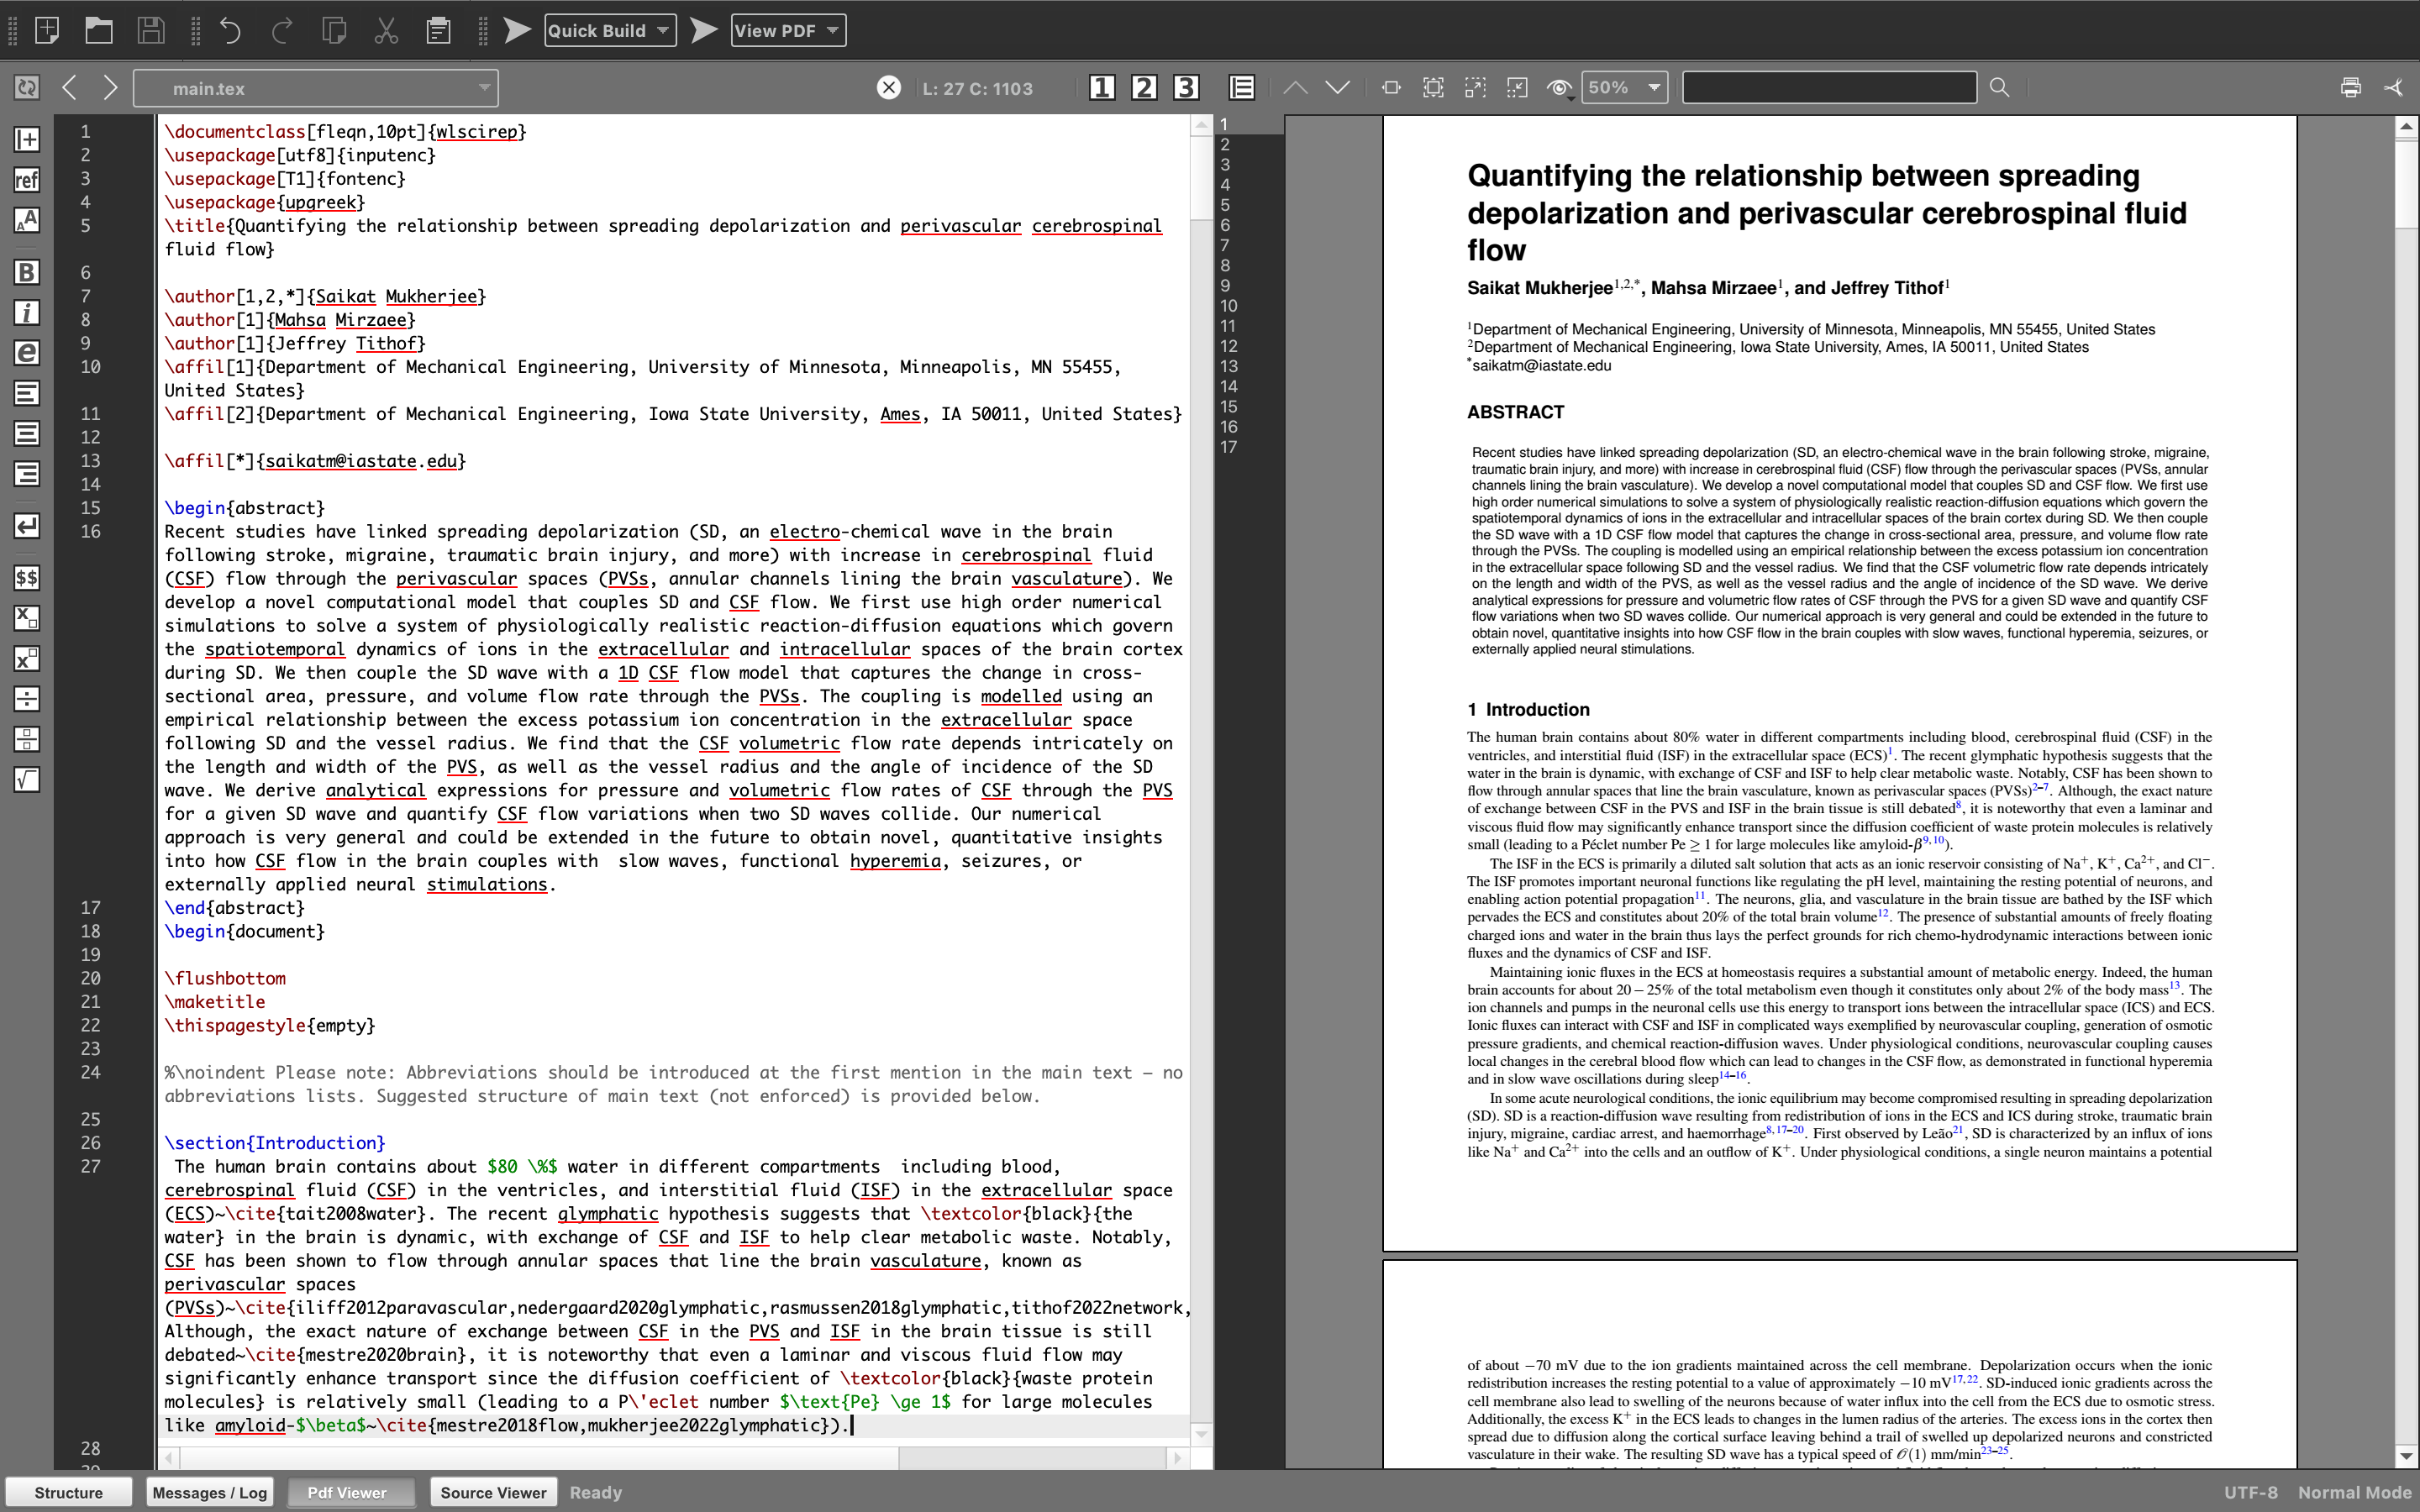
\includegraphics[width=0.8\linewidth]{latex_example.png}
    %\caption{Enter Caption}
    \label{fig:enter-label}
\end{figure}   

\end{frame}

% Pros slides
\begin{frame}{Accepted by Academic Journals}
    Preferred by many.
    \begin{example}
        
\includegraphics[width=0.5\linewidth]{nature.jpg}
    \end{example}

\end{frame}

\begin{frame}{Professional Typesetting and Templates}
    Focus on content. Let \LaTeX\ render and organize the rest. Choose from built-in modules and templates. 
    \begin{example}
    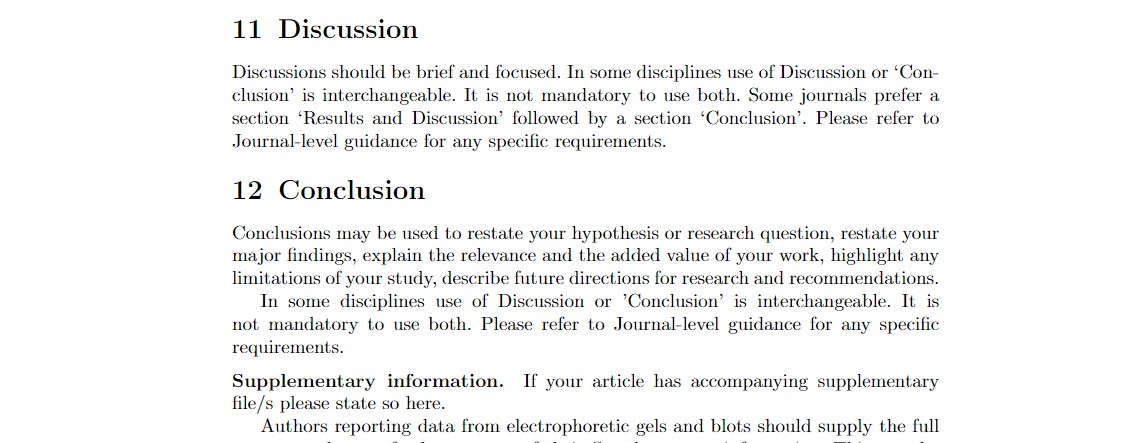
\includegraphics[width=\textwidth]{nature_paper_pic.jpg}
    
    % like this \lstinline{example} environment in the presentation document class \lstinline{Beamer}. 
    \end{example}
\end{frame}
\begin{frame}{Powerful mathematics typesetting}
Subscripts, fractions, multi-line equations, matrices, accents (vector, bar, hat)
\begin{example}
    $$
\mathbf{J}
=
\frac{d \mathbf{f}}{d \mathbf{x}}
=
\left[ \frac{\partial \mathbf{f}}{\partial x_1}
\cdots \frac{\partial \mathbf{f}}{\partial x_n} \right]
=
\begin{bmatrix}
\frac{\partial f_1}{\partial x_1} & \cdots &
\frac{\partial f_1}{\partial x_n} \\
\vdots & \ddots & \vdots \\
\frac{\partial f_m}{\partial x_1} & \cdots &
\frac{\partial f_m}{\partial x_n}
\end{bmatrix}
$$
\end{example}
% \begin{example}
%    Inline rendering, such as $e=mc^2$
% \end{example}
% or
% \begin{example}{Display Style}
%     Display style (and auto-numbered)
%     \begin{equation}
%         F = G \cdot \frac{m_1 \cdot m_2}{r^2}
%     \end{equation}
% \end{example}
% \begin{example}
%     % \begin{equation}
%         $\left|\frac{X}{Y}\right|={\left(\frac{{\left(1+\left(4\zeta^2 -1\right)r^2 \right)}^2 +{\left(2\zeta r^3 \right)}^2 }{{\left(1-r^2 \right)}^2 +{\left(2\zeta \;r\right)}^2 }\right)}^{\frac{1}{2}}$
%     % \end{equation}
%     % \begin{equation}
%             $\phi ={\mathrm{tan}}^{-1} \left(\frac{-2\zeta r^3 }{1+\left(4\zeta^2 -1\right)r^2 }\right)$
%     % \end{equation}
% \end{example}
% \begin{example}
% $
% A = 
% \left[\begin{array}{cc}
% m\,L^2 \,\cos^2\theta +m\,L^2 \,{\sin}^2\theta +J & L\,m\,\cos \theta\\
% L\,m\,\cos \theta & M+m
% \end{array}\right]$
% % , $
% % M=\left[\begin{array}{c}
% % 0\\
% % L\,m\,\sin \theta\,{\dot{\theta}}^2 -2\,K\,x
% % \end{array}\right]$
% % \end{equation*}
% \end{example}
\begin{example}
    % \begin{equation}
% \frac{\partial \rho}{\partial t} + \overrightarrow{\nabla}\cdot(\rho\overrightarrow{u})=0 \end{equation}
\begin{equation}
\frac{\partial(\rho \overrightarrow{u})}{\partial t} + \overrightarrow{\nabla}\cdot[\rho\overline{\overline{u\otimes u}}] = -\overrightarrow{\nabla p} + \overrightarrow{\nabla}\cdot\overline{\overline{\tau}} + \rho\overrightarrow{f} \end{equation}
\begin{equation}
\frac{\partial(\rho e)}{\partial t} + \overrightarrow{\nabla}\cdot((\rho e + p)\overrightarrow{u}) = \overrightarrow{\nabla}\cdot(\overline{\overline{\tau}}\cdot\overrightarrow{u}) + \rho\overrightarrow{f}\overrightarrow{u} + \overrightarrow{\nabla}\cdot(\overrightarrow{\dot{q}})+r \end{equation}

\end{example}
\end{frame}

\begin{frame}[fragile]{Embed code snippets}\label{slide:code}
    Use the \lstinline|listings| package to embed code snippets.
    \begin{example}
      \begin{lstlisting}[mathescape]
    \begin{equation}\label{eq:example}
        F = G \cdot \frac{m_1 \cdot m_2}{r^2}
    \end{equation}
    \end{lstlisting} will render this popular equation \cite{einstein1905}
    \begin{equation}\label{eq:example}
        F = G \cdot \frac{m_1 \cdot m_2}{r^2}
    \end{equation}
    
    \end{example}
    
\end{frame}
\begin{frame}{Cross-Referencing}
    \LaTeX\ enables accurate cross-referencing of figures, tables, equations, and sections, maintaining consistency and reducing errors.\\ \vspace{0.2in}
    Basic idea: each figure, table, etc. gets a label, then that label can be referenced without manually keeping track of figure/table/etc. count\\
    \vspace{0.2in}
        
    \begin{example}
        Equation~(\ref{eq:example}) from slide \ref{slide:code} [Click to follow].
    \end{example}
\end{frame}

\begin{frame}{Version Control}
   Plain text files and nested folder organization. Never lose a figure you changed your mind about.\\
   \vspace{0.2in}
    
    \begin{example}
    \begin{itemize}
        \item Project can be tracked on Git/github
        \item Overleaf also supports collaboration [free] and change-tracking [paid]
    \end{itemize}
    \end{example}
\end{frame}

\begin{frame}{Customization}
\begin{columns}
    \begin{column}{0.5\textwidth}
     Extensive customization through templates, fonts, styles
        \begin{example}
        \begin{itemize}
            \item Embed code snippets with \lstinline{listings}
            \item Insert pdfs [e.g. your transcript] with \lstinline{pdfpages}
            \item Vector graphics using \lstinline{svg} such as in Figure \ref{fig: svg}
            \item Modular organization through separate files; choose sections to include/exclude
        \end{itemize}
        \end{example}
    \end{column}
    \begin{column}{0.5\textwidth}
    \begin{figure}
        \centering
        \includesvg[width=\textwidth]{CW_full_small2}
        \caption{SVG rendered and captioned in LaTeX}
        \label{fig: svg}
    \end{figure}
    \end{column}
   
    \end{columns}
    
\end{frame}

% \begin{frame}{Modular organization}
%     Keep different sections in separate .tex files and include/exclude them in your document (and future documents) with ease
%     \begin{example}
%         \begin{lstlisting}
%             \input{section_about_propulsion}
%             \input{section_about_gravity}
%         \end{lstlisting}
%     \end{example}
% \end{frame}

% \begin{frame}{Community and Templates}
%     \LaTeX\ has a vast community, providing resources, templates, and packages that simplify tasks and enhance document appearance.
    
%     \begin{example}
%         Utilize \LaTeX\ templates for presentations, research papers, CVs, and more, shared by the community.
%     \end{example}
% \end{frame}

\begin{frame}{References}\label{slide:references}
Finally, it's super-simple to embed and format citations \cite{latexcompanion}
\begin{example}
    \bibliographystyle{ieeetr}
    \bibliography{example_bib}
\end{example}
\end{frame}

% Cons slide
\begin{frame}{Cons}
    \begin{itemize}
        \item Learning Curve
        \item Real-Time Collaboration
        \item Customization Complexity
        \item Document Maintenance
        \item Complicated tables
        \item No universal distributor
        \item Some collaborators may be completely unwilling to use
    \end{itemize}

    \vspace{0.2in}
    
    However:\\
    \begin{itemize}
    \item Overleaf (includes ShareLaTeX) offers real-time collaborative document generation, revision history, cloud sync
    \item Free online resources are available for easily generating tables
    \end{itemize}
\end{frame}

% Cons slide
\begin{frame}{Do we recommend the software for...}
    \begin{itemize}
        \item reports, homework, projects?
        \begin{itemize}
            \item[--] Perhaps. It's probably not worth learning from scratch unless the assignment is very math intensive.
        \end{itemize}
        \item publications?
            \begin{itemize}
                \item[--] Yes! Especially if your advisor and/or collaborators agree.
            \end{itemize}
        \item written prelim exam?
            \begin{itemize}
                \item[--] Yes! And there is a template you can use.
            \end{itemize}
        \item thesis/dissertation?
            \begin{itemize}
                \item[--] Yes! We \textbf{highly recommend} doing so since you'll have many chapters, figures, tables, etc. that may be shuffled during writing. 
            \end{itemize}
        \item grant proposals?
            \begin{itemize}
                \item[--] Yes! But only if your collaborators agree.
            \end{itemize}
    \end{itemize}
\end{frame}
    
\end{document}
